%=================== LaTeX 习题模板(仅含学院与考试信息) ===================
\documentclass[12pt,a4paper]{article}

%----------------- 页面与中文支持 -----------------
\usepackage[margin=2cm]{geometry}    % 设置页边距
\usepackage{ctex}                    % 支持中文
\usepackage{amsmath,amssymb}         % 数学公式与符号
\usepackage{enumitem}                % 自定义列表格式
\usepackage{tikz}
\usetikzlibrary{decorations.pathmorphing}
\usepackage{float} % 支持 [H] 浮动体选项

%----------------- 页眉页脚 -----------------
\usepackage{fancyhdr}
\pagestyle{fancy}
\fancyhf{}
% 左侧:学院(留空由学生填写)
\lhead{学院:\underline{\hspace{2cm}建工学院\hspace{2cm}}}
% 右侧:考试信息(如“期末考试”、“月考试卷”等,由学生填写)
\rhead{考试:\underline{\hspace{2cm}测量学\hspace{2cm}}}
\cfoot{\thepage}

%----------------- 题目环境 -----------------
\newcounter{question}
\newenvironment{questions}{
    \setcounter{question}{0}
    \section*{习题(题目)}
    \begin{enumerate}[leftmargin=1.5em,label={\arabic*.}]
}{
    \end{enumerate}
}

%----------------- 答案环境 -----------------
\newenvironment{answers}{
    \setcounter{question}{0}
    \section*{习题答案}
    \begin{enumerate}[leftmargin=1.5em,label={\arabic*.}]
}{
    \end{enumerate}
}

% 用于每题答案的加粗提示
\newcommand{\answer}[1]{\par\noindent\textbf{答案:} #1\par\vspace{1em}}

%=========================================================

\begin{document}



\newpage

%=================== 题目部分 ===================
\section*{第一章\quad 测量基础知识}
\begin{questions}
    \item 大地水准面的概念及作用是什么?
    \answer{大地水准面是与假想的处于流体静平衡状态的海洋面相重合并延伸到大
陆的重力等位面。它的作用是作为测量高程的基准面。}
    \item 地面点位的确定用什么方法?测量上的平面直角坐标系有哪几种?它和数学上的平面直角坐标系有什么区别?为什么要规定测量平面直角坐标系的象限按顺时针方向编号?
    \answer{地面点位的确定采用多种坐标系方法,包括地球空间直角坐标系、球面和平面坐标系(含地理坐标系、平面直角坐标系)}
    \answer{测量学里的平面直角坐标系包括,高斯直角坐标系、独立平面坐标系。区别是顺时针依次为第一、第二、第三、第四象限,而数学上的平面直角坐标系是逆时针依次为第一、第二、第三、第四象限。规定测量平面直角坐标系的象限按顺时针方向编号是为了与全站仪测量时旋转方向一致(全站仪顺时针旋转为正),便于实际应用。}
    \item 什么是绝对高程和相对高程?在什么情况下可采用相对高程?
    \answer{绝对高程是指某点相对于大地水准面的高度,而相对高程是指某点相对于另一个已知点的高度差。当测区附近无国家水准点,而引测绝对高程有困难时,
可以采用假定高程系统,即假定一个水准面作为高程基准面}
    \item 用水平面代替球面对距离和高程有什么影响?在多大范围内可用水平面代替球面?为什么?
    \answer{用水平面代替球面对距离和高程的影响主要体现在测量精度上。水平面假设会导致测量结果在大范围内产生误差,尤其是高程测量(高程测量一般不能忽略曲率)。通常在小于数十公里的范围内可以近似使用水平面代替球面,因为此时地球曲率对测量结果的影响较小。}
    \item 测量工作的基本原则是什么?有什么作用?
    \answer{在布局上从整体到局部,在程序上先控制后碎部,在作业上步步有检核 }
    \item 确定地面点位的三项基本测量工作是什么?
    \answer{确定地面点位的三项基本测量工作是:距离测量、角度测量及高程测量}
\end{questions}

\section*{第一章\quad知识点补充}
测量学的基本任务:地形图测绘,地形图应用,施工测量,变形观测。 

我国目前使用的坐标系为2008年7月1日启用的2000国家大地坐标系。我国目前的高程基准为“1985 国家高程基准”,其水准原点高程为
72.2604 米,全国各地的高程都以它为基准进行测算。

    \begin{figure}[H]
        \centering
        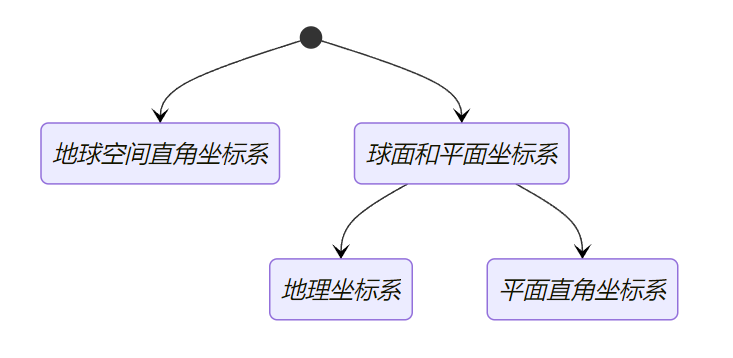
\includegraphics[width = 0.6\textwidth]{./figures/6.png}
    \end{figure}

地球空间直角坐标系使用的三维坐标(x,y,z),一般建在地球的质心,美国的GPS
所采用的WGS-84坐标系也属于地心空间直角坐标系。

球面和平面坐标系采用的是先定位在参考椭球上的位置,再定位高程,最终定位点。

和第一种的区别是,(1)原点为参考椭球中心\quad (2)采用了分解的思想,可以通过最小二乘法反算

\begin{enumerate}
    \item 大地高系统——是地面点沿参考椭球面法线到参考椭球面的距离。
    \item 正高系统——是地面点沿重力线到大地水准面的距离。
    \item 正常高系统——是地面点沿正常重力线到似大地水准面的距离。
\end{enumerate}
三者的区别是大地高系统是到参考椭球面的,正高是到大地水准面的(大地水准面的水准面是不均匀非理想的几何体,有无数个水准面),而正常高
是沿着正常重力线的(解释下正常重力线不是真实存在的,是将重力场近似为椭球体),我国采用正常高系统。
\newpage

\section*{第二章\quad 水准测量}
\begin{questions}
    \item 设 \( A \) 为后视点,\( B \) 为前视点,\( A \) 点高程为 93.533 米,当后视读数为 1.025 米,前视读数为 1.674 米时,高差是多少?\( B \) 点比 \( A \) 点高还是低?\( B \) 点高程是多少?绘图说明。
    
    高差计算公式(a为后视读数,b为前视读数):
    $$h_{AB} = a - b$$

    \answer{高差 \( h_{AB} = 1.025 - 1.674 = -0.649 \) 米,说明 \( B \) 点比 \( A \) 点低。\( B \) 点高程为 \( 93.533 - 0.649 = 92.884 \) 米。绘图如下(仿照课本标准图画下就行)}
    \begin{figure}[H]
        \centering
        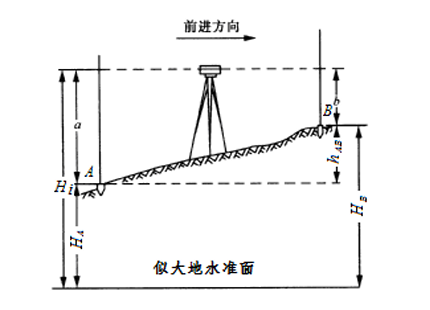
\includegraphics[width = 0.7\textwidth]{./figures/1.png}
        \caption{水准测量示意图}
    \end{figure}
    \item 何谓视准轴?何谓视差?产生视差的原因是什么?怎样消除视差?
    \answer{视准轴是十字丝交点与物镜光心的连线。视差是指望远镜视准轴与被测点之间的偏差。产生视差的原因主要是,眼睛观察时,视线通过目镜看到的十字丝和尺子成像焦点不在同一平面,显然这会导致读数会随视线移动发生变化。消除视差的方法为对目镜和物镜调焦,直至视线移动时成像也保持不变,可以读到清晰读数。}
    \item 水准测量时为什么要求前、后视距相等?
    \answer{水准测量时要求前、后视距相等是为了消除$i$角误差。通过保持前后视距相等,可以使得测量结果更为准确,减少系统误差的影响。}
    \item 水准仪有哪些轴线?它们之间应满足哪些条件?其中主要条件是什么?
    \answer{包括视准轴 CC、水准管轴 LL、仪器竖轴 VV、圆水准器轴 L'L'}
    满足条件:

(1) 视准轴 CC// 水准管轴 LL(主条件)

(2) 仪器竖轴 VV// 圆水准器轴 L'L'

(3) 十字丝横丝 ⊥ 仪器竖轴(十字丝横丝应水平)

    \item 已知 \( BM_A \) 点的高程为 44.218 米,将下图中的水准测量观测数据填入记录手簿(见下表),计算出各点的高差及 \( B \) 点的高程,并进行计算检核。
    \begin{figure}[H]
        \centering
        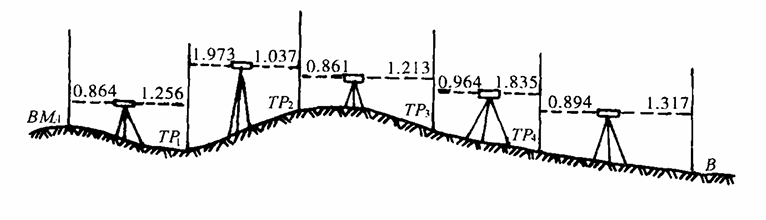
\includegraphics[width = 0.7\textwidth]{./figures/2.png}
        \caption{水准测量观测数据}
    \end{figure}
    \answer{太简单了,同上,计算检验就是总后视减去总前视}
    对于一般的水准测量,计算检验公式为:
    \begin{enumerate}
    \item 闭合水准路线:$f_h = \sum h_{\text{测}}$
    \item 附合水准路线:$f_h = \sum h_{\text{测}} - (H_{\text{终}} - H_{\text{始}})$
    \item 支水准路线:$f_h = \sum h_{\text{往}} + \sum h_{\text{返}}$
\end{enumerate}

    \item 下图为一五等水准路线的观测结果, $BM_A$ 高程为 15.617 米,试在下表中完成成果计算。
    \begin{figure}[H]
        \centering
        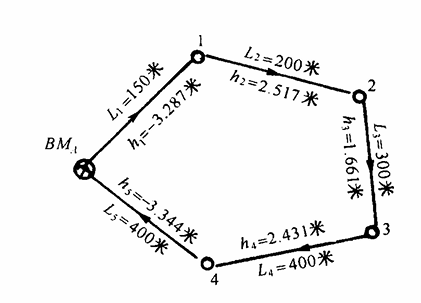
\includegraphics[width = 0.4\textwidth]{./figures/5.png}
    \end{figure}

    \begin{figure}[H]
        \centering
        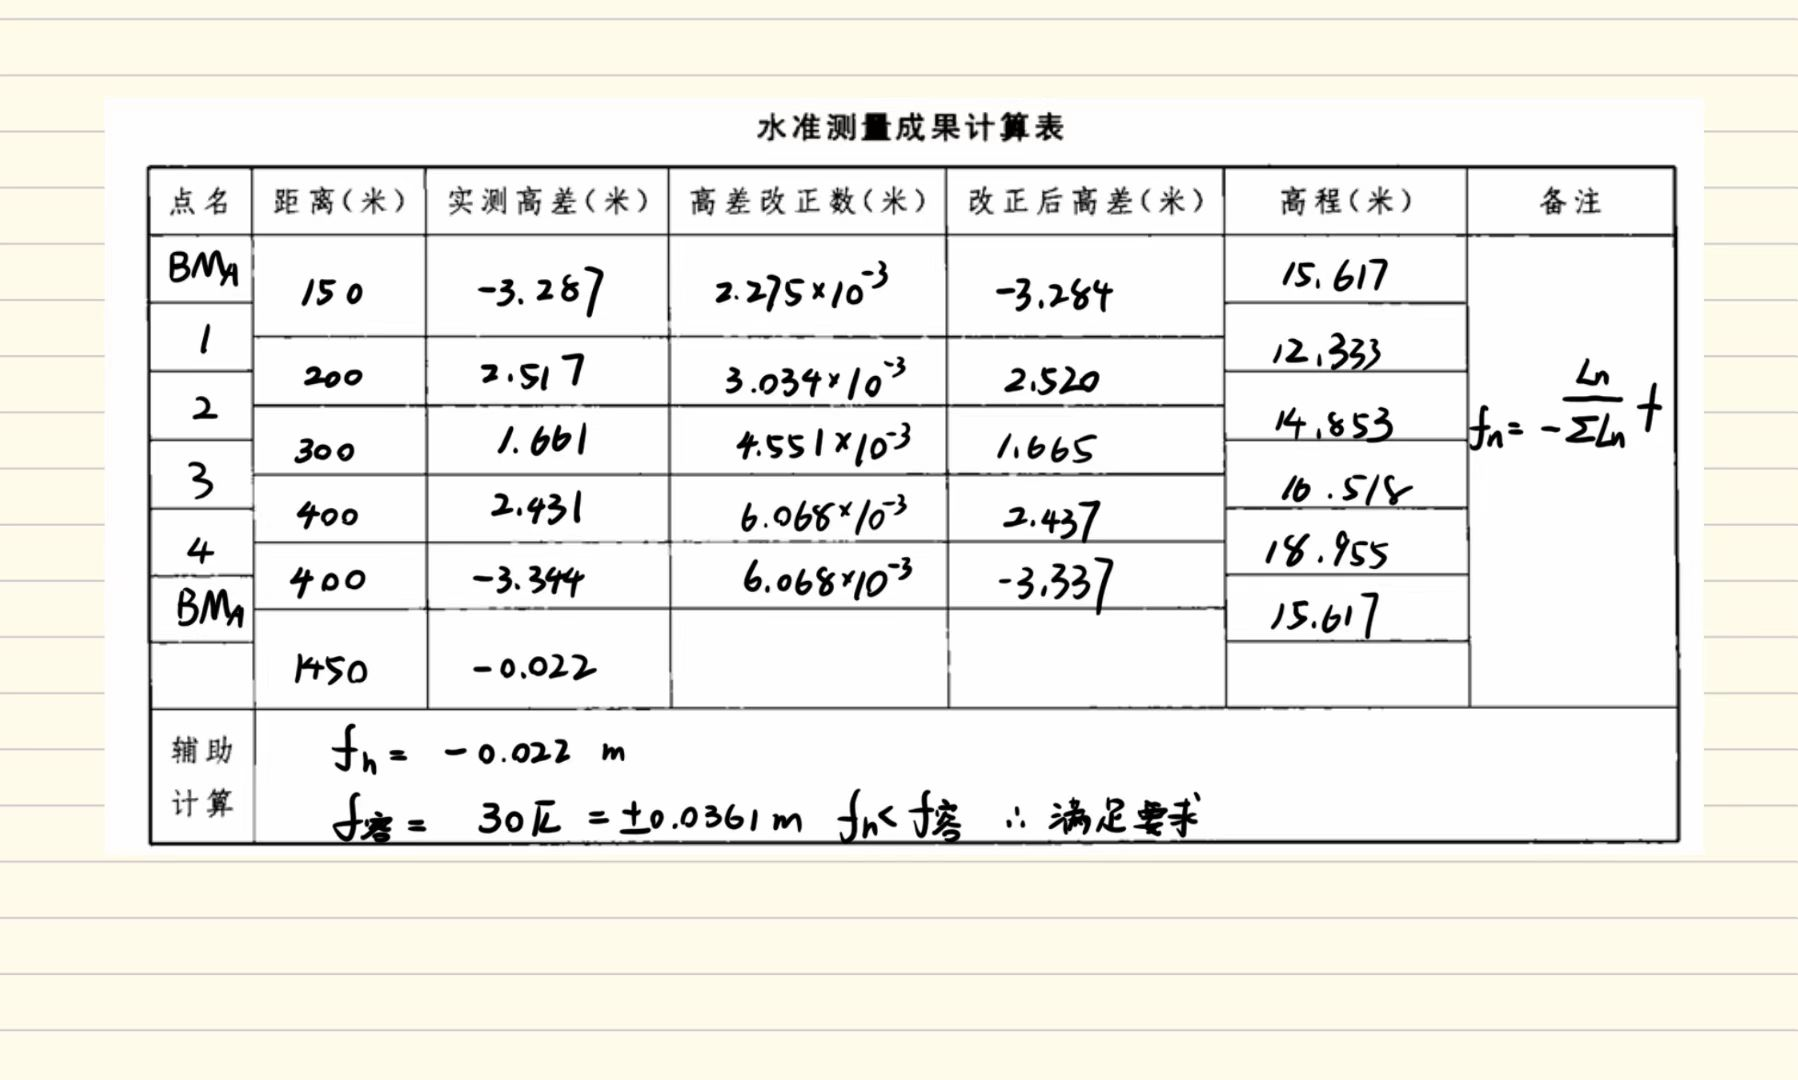
\includegraphics[width = 0.9\textwidth]{./figures/6.jpg}
    \end{figure}
    {\color{red}注意,这里$L$单位是km}
\end{questions}

\section*{第二章\quad知识点补充}

水准仪的类型:水准仪按结构可分为{\color{red}微倾式水准仪、自动安平水准仪和数字水
准仪}。

DS3微倾式水准仪的操作程序:安置、粗平、瞄准、精平、读数。 

水准测量原理:水准测量是利用水准仪提供的水平视线在水准尺上读数,测得
地面两点间的高差,进而由已知点高程推算出未知点高程。

\subsection*{水准测量的误差来源}
\begin{enumerate}
    \item 仪器误差:包括仪器 $i$ 角误差(可通过调整前后距离相同消除)、水准尺误差。
    \item 观测误差:包括整平误差、读数误差、水准尺倾斜误差。
    \item 外界条件的影响:包括仪器和尺子下沉、地球曲率和大气折光的影响、温度、风力等外界条件的影响。
\end{enumerate} 
\newpage

\section*{第三章\quad 角度测量}
\begin{questions}
    \item 经纬仪有哪几条轴线?经纬仪应满足哪些几何条件?
    \answer{经纬仪有视准轴CC、十字丝横轴HH、水准管轴LL、竖轴VV。经纬仪应满足以下几何条件:

    (1)CC ⊥ HH

    (2)LL ⊥ VV

    (3)HH ⊥ VV

    (4)纵丝 ⊥ HH

    (5)竖盘指标处于正确位置(x=0)

    (6)光学对中器的视准轴与竖轴重合}

    \item 用盘左、盘右两个位置观测水平角能消除哪些误差?
    \answer{通过盘左、盘右两个位置观测水平角,可以消除仪器的偏心误差和视准轴的倾斜误差。}    

    \item 完成半测回和一测回角度表格
    
    \answer{半测回由盘右读数相减以及盘左读数相减得到,计算公式为:
\[
\beta_{\text{左}} = b_{\text{左}} - a_{\text{左}},\beta_{\text{右}} = b_{\text{右}} - a_{\text{右}}
\]

上、下半测回合称一测回。对于 DJ6 型经纬仪,要求:\(\beta_{\text{左}}\)与\(\beta_{\text{右}}\)的差值不大于 \(40''\),如符合要求,则取盘左盘右的平均值作为观测结果。
\[
\beta = \frac{1}{2} (\beta_{\text{左}} + \beta_{\text{右}})
\]}

    \item 根据下表记录,计算竖直角和指标差。
    
    \answer{对于竖直角测量,盘左、盘右的竖直角计算分别为 \(\alpha_{\text{左}}\) 和 \(\alpha_{\text{右}}\),则竖直角计算公式为:
    $$\alpha _ { L } = 9 0 ^ { \circ } - L + x,\alpha _ { R } = R - 270 ^ { \circ } - x$$
    其中 \(L\) 为盘左读数,\(R\) 为盘右读数,\(x\) 为指标差。指标差的计算公式为:
    $$x = \frac{1}{2} (L + R - 360^\circ)$$
    这就是为什么说盘左加盘右的测量可以消除指标误差。
    }
\end{questions}

\section*{第三章\quad 知识点补充}
水平角:一点到两个目标点的方向线垂直投影到水平面上所形成的夹角。水平
角的角值范围在0~360°之间。 

竖直角:观测目标的方向线与同一铅垂面内的水平线之间的夹角,也称为垂直
角。竖直角有正负之分,仰角为正,俯角为负,角值范围在0~±90°之间。 

经纬仪按测角原理可分为{\color{red}光学经纬仪和电子经纬仪}。

\newpage

\section*{第四章\quad 距离测量}
\begin{questions}
    \item 在钢尺量距中为什么要进行直线定线?
    \answer{有时候钢尺量距时,测量线段可能会受到障碍物的影响,也有可能因为钢尺长度不够,导致无法直接测量。直线定线可以通过设置标志点或使用导向杆等方式,确保测量线段的直线性,从而提高测量精度。}
    \item 根据表中所给各碎部点的观测记录,在表上计算相应的距离及高程(测站高程 \( H_0 = 25.47 \) 米,仪器高 \( i = 1.47 \) 米,盘左时 \( \alpha = 90^\circ - L \))。
    \begin{figure}[H]
        \centering
        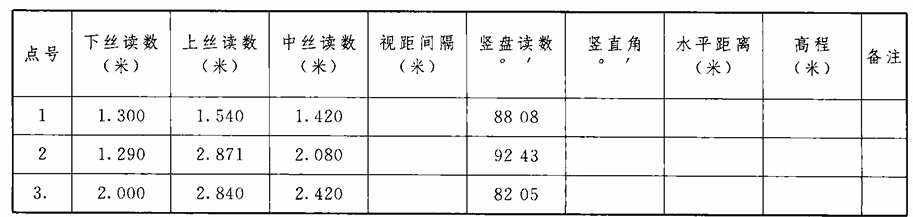
\includegraphics[width = 0.7\textwidth]{./figures/3.png}
        \caption{水准测量观测数据}
    \end{figure}
    \answer{
        视距间隔=上丝读数-下丝读数,竖直角=盘左读数-90°

        水平距离=$Kncos^2(\alpha)$
    
        高差=$\frac{1}{2}Knsin(2\alpha) + i - l$
        
        K是仪器参数,一般取为100,n为视距间隔,i为仪器高,l为中丝读数,记得加上测站高程(题目问的是高程)
    }

    \item 全站仪主要由哪几部分组成?
    
    \answer{全站仪主要由电子测角、光电测距和数据微处理系统组成。全站仪是全站型电子速测仪的简称,它能在一个测站上同时完成角度测
量和距离测量。}

    \item 用钢尺丈量 \(A\)、\(B\) 两点距离,设往测为 127.432 米,返测为 127.467 米,相对误差为多少?
    \answer{
    理论依据:量距相对误差的定义为,往返丈量的距离之差的绝对值与平均距离之比,并化成分子为
1 的形式,用于衡量丈量结果的精度。其中,平坦地区钢尺量距的相对误差不应大于1/3000;在量距困难地区,
其相对误差也不应大于1/1000。

    相对误差计算公式为:
    
    相对误差= $\frac{\text{绝对误差}}{\text{真值}} \times 100\%$

    其中,绝对误差=往测-返测=|127.432-127.467|=0.035 米
    
    真值=(往测+返测)/2=(127.432+127.467)/2=127.45 米
    }
\end{questions}

\section*{第四章\quad 知识点补充}

视距测量是用望远镜内的视距装置,根据光学和三角学原理测定距离和高差的
一种方法。特点是操作简便、速度快,不受地形的限制,但测距精度较低,一般相对
误差为1/300~1/200,测高差的精度也低于水准测量和三角高程测量。它主要用于地
形图的碎部测量。 

根据测量电磁波传播时间的方法的不同,电磁波测距仪可以分为脉冲式测距仪
和相位式测距仪。 

    \begin{figure}[H]
        \centering
        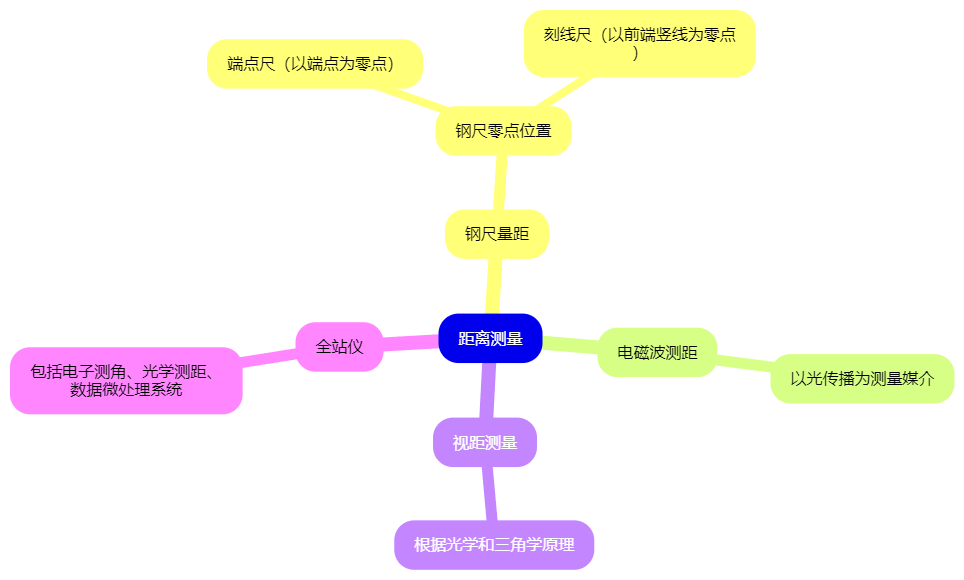
\includegraphics[width = 0.9\textwidth]{./figures/8.png}
    \end{figure}
    

\section*{第五章\quad 测量误差及测量平差}

\begin{questions}
    \item 试述偶然误差的主要特性。
    
    \answer{偶然误差是指在测量过程中由于各种随机因素引起的误差,其主要特性包括:
        \begin{enumerate}
\item 在一定的观测条件下,偶然误差的绝对值不会超过一定的限值。

\item 绝对值较小的误差比绝对值较大的误差出现的机会多。

\item 绝对值相等的正、负误差出现的机会均等。

\item 偶然误差的算术平均值随观测次数的无限增加而趋向于零
    \end{enumerate}}


    

    \item 写出用观测值的真误差和观测值的改正数计算中误差的公式,并说明各自的适用情况。
    \answer{已知真误差计算中误差的计算公式为:
    $$m = \sqrt{\frac{\sum_{i=1}^{n} v_i^2}{n}}$$
    只知道观测值计算改正数的中误差计算公式:
    $$m = \sqrt{\frac{\sum_{i=1}^{n} v_i^2}{n - 1}}$$
    }

    \item 设对某一水平角观测了9个测回,观测值为:130°25′18″, 130°25′30″, 130°25′12″, 130°25′24″, 130°25′06″, 130°25′18″, 130°25′24″, 130°25′12″, 130°25′06″,求该角的最可靠值、观测值中误差和算术平均值中误差。
    \answer{最可靠值就是平均数,观测值中误差就是参考上一题的第二个公式:
    $$m = \sqrt{\frac{\sum_{i=1}^{n} v_i^2}{n - 1}}$$
    算术平均数的中误差是由误差传播公式导出:
    $$M = \frac{m}{\sqrt{n}}$$
    }
    \item 已知观测角度一个测回的中误差为±8″.5,欲使测角精度提高一倍,问应观测几个测回?
    \answer{由上文的算术平均数的中误差公式可知:应当测4次,然后取平均数。}

    \item 观测一个四边形的三内角,中误差分别为士10"、士8"和士6",求第四个内角的中误差?
    \answer{由误差传播公式以及线性函数时的误差传播公式可知:
    $$m = \sqrt{m_1^2 + m_2^2 + m_3^2}$$
    注:这里的角度计算公式为:$$\alpha = 360^\circ - \alpha_1 - \alpha_2 - \alpha_3$$
    }
\end{questions}

\section*{第五章\quad 知识点补充}

\begin{figure}[H]
    \centering
    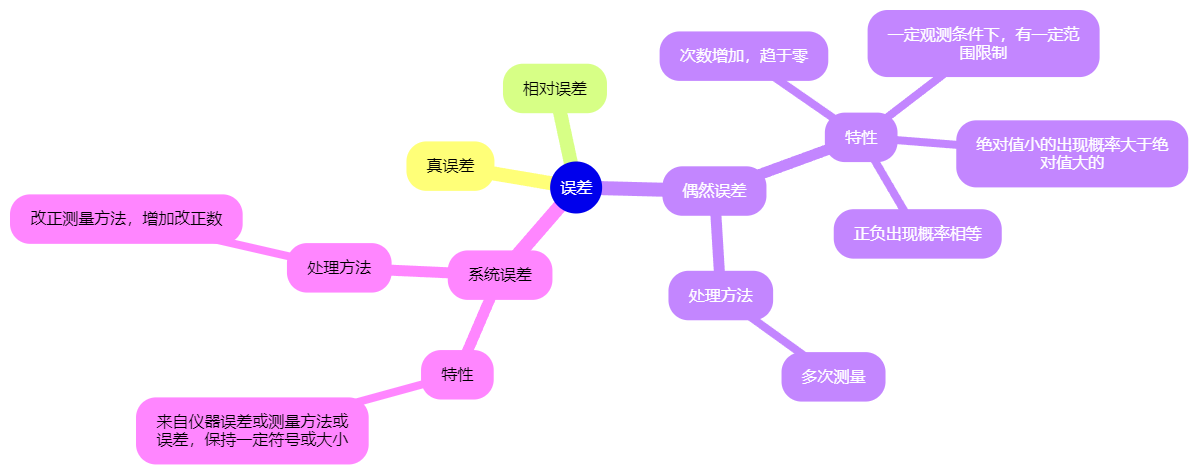
\includegraphics[width = 0.8\textwidth]{./figures/7.png}
    \caption{测量误差的分类}
\end{figure}

研究测量误差的目的在于:分析测量误差的产生原因、性质和积累规律;正确
地处理观测结果,求出最可靠值;评定测量结果的精度;通过研究误差发生的规律,
为选择合理的测量方法提供理论依据。 

\newpage

\section*{第六章\quad 定向测量}

\begin{questions}
    \item 测量上作为定向依据的标准方向有哪些?什么叫方位角?
    \answer{包括真子午线方向、磁子午线方向、平面直角坐标系的 X 轴方向等。方位角是指从北向东测量的角度,用来表示某一方向相对于北方的偏离程度。}
    \item 某五边形的各内角 $\beta_1=90^\circ$, $\beta_2=130^\circ$, $\beta_3=70^\circ$, $\beta_4=128^\circ$, $\beta_5=122^\circ$,各角与点号对应,各点按逆时针方向编号,已知 1~2 边的坐标方位角为 $30^\circ$,求其他各边的坐标方位角。
\answer{
方向角计算公式为:
\[
\text{左角: }\quad \alpha_{\text{前}} = \alpha_{\text{后}} + \beta_{\text{左}} - 180^\circ
\]
\[
\text{右角: }\quad \alpha_{\text{前}} = \alpha_{\text{后}} - \beta_{\text{右}} + 180^\circ
\]
这里因为给的是内角,同时是逆时针方向,所以可以直接使用左角公式计算。
}

\item 已知 \(A\)、\(B\) 两点的坐标为 \(x_A = 697.54\) 米, \(y_A = 1248.52\) 米, \(x_B = 1295.24\) 米, \(y_B = 866.44\) 米, 求 \(AB\) 的边长及方位角。

\answer{注意这里测量学的坐标系特点,方位角计算公式如下:
$$D = \sqrt{(x_B - x_A)^2 + (y_B - y_A)^2}
$$
$$\alpha_{AB} = \arctan \frac{y_B - y_A}{x_B - x_A}$$
\begin{figure}[H]
        \centering
        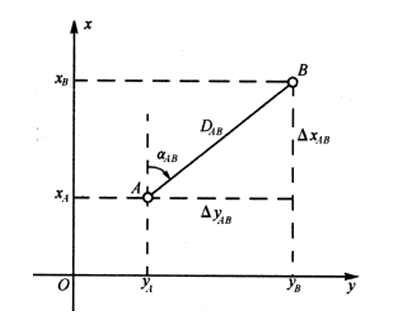
\includegraphics[width = 0.4\textwidth]{./figures/4.png}
        \caption{水准测量观测数据}
    \end{figure}
}
\end{questions}

\section*{第六章\quad 知识点补充}

标准方向的种类:真子午线方向、磁子午线方向、坐标纵轴方向。根据标准方
向线的不同,方位角分为真方位角、磁方位角和坐标方位角。 

\begin{enumerate}
    \item 真子午线方向:通过天文观测确定的地理子午线方向,通常以地球自转轴为基准,精度高,受地理位置影响。
    \item 磁子午线方向:以磁针静止时指向的方向为基准,受地磁场影响,存在磁偏角,易于现场快速定向。
    \item 坐标纵轴方向:以平面直角坐标系的X轴(或Y轴)为基准方向,常用于大地测量和工程测量中的坐标方位角计算。
\end{enumerate}

\newpage

\section*{第七章\quad 小地区控制测量}

\begin{questions}
    \item 小地区控制的导线有哪几种布设形式?
    \answer{包括闭合导线、附合导线和支导线。闭合导线是指起点和终点重合的导线,附合导线是指起点和终点不重合但有已知点连接的导线,支导线是指从已知点向外延伸的导线。}
    \item 闭合导线与附合导线在计算过程中有哪些异同?
    \answer{
        闭合导线是从一个已知边的一个已知点出发,经过一系列导线点,最后
仍回到起始点。附合导线是从一个已知边的一个已知点出发,经过一系列导线点,最后
附合到另一已知边的一个已知点上。 支导线没有检核条件,不易发现错误,一般用于难以布设闭合或附合导
线的狭长地带及困难地区。

两种导线的坐标计算方法类似,但是在角度闭合差和坐标闭合差的计算上有不同。

对于闭合导线:
\[
\sum \beta_{\text{测}} = \beta_1 + \beta_2 + \cdots + \beta_n
\]
\[
\sum \beta_{\text{理}} = (n - 2) \cdot 180°
\]
\[
f_{\beta} = \sum \beta_{\text{测}} - \sum \beta_{\text{理}}
\]
若 \( f_{\beta} \leq f_{\beta_{\text{容}}} \),则进行角度闭合差调整:反符号平均分配。

改正数 \( V_{\beta} \) 为:
\[
V_{\beta} = -\frac{f_{\beta}}{n}
\]
导线全长闭合差:
\[ f = \sqrt{f_x^2 + f_y^2},f_x = \sum x ,f_y= \sum y \]
导线相对闭合差:
\[ T = \frac{f}{\sum D} = \frac{1}{\sum D} \cdot \frac{1}{f} \]

对于附和导线:

(1) 角度闭合差的计算

对左侧角: \(\sum \beta_{\text{左测}} = \alpha_{\text{终}} - \alpha_{\text{始}} + n \cdot 180^\circ\)

对右侧角: \(\sum \beta_{\text{右测}} = \alpha_{\text{始}} - \alpha_{\text{终}} + n \cdot 180^\circ\)

\(f_{\beta} = \sum \beta_{\text{测}} - \sum \beta_{\text{理}}\)

(2) 坐标增量闭合差的计算

\(\sum \Delta x_{\text{理}} = x_{\text{终}} - x_{\text{始}}\)

\(\sum \Delta y_{\text{理}} = y_{\text{终}} - y_{\text{始}}\)

\(f_{x} = \sum \Delta x_{\text{测}} - \sum \Delta x_{\text{理}} = \sum \Delta x_{\text{测}} - (x_{\text{终}} - x_{\text{始}})\)

\(f_{y} = \sum \Delta y_{\text{测}} - \sum \Delta y_{\text{理}} = \sum \Delta y_{\text{测}} - (y_{\text{终}} - y_{\text{始}})\)
}
\item 已知一条图根闭合导线 $1,2,3,4,1$,方位角 $\alpha_{12} = 64^\circ 30' 45''$,观测了 4 个内角(右角)分别为:$\angle 1 = 86^\circ 18' 06''$,$\angle 2 = 86^\circ 25' 37''$,$\angle 3 = 89^\circ 36' 23''$,$\angle 4 = 97^\circ 39' 54''$,4 条边长为:$D_{12} = 177.970\,\text{m}$,$D_{23} = 138.003\,\text{m}$,$D_{34} = 161.822\,\text{m}$,$D_{41} = 126.924\,\text{m}$,且 1 号点的坐标 $x_1 = 610.148\,\text{m}$,$y_1 = 813.818\,\text{m}$,求各点的坐标。

\answer{使用上题的闭合导线计算方法}

\item GNSS 由哪几部分组成?
\answer{GNSS由空间卫星、地面监控系统和用户接收机三部分组成。}
\end{questions}

\section*{第九章\quad 知识点补充}
\begin{figure}[H]
    \centering
    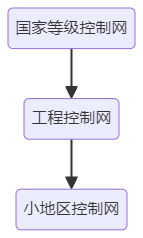
\includegraphics[width=0.15\textwidth]{./figures/9.png}
    \hspace{1cm}
    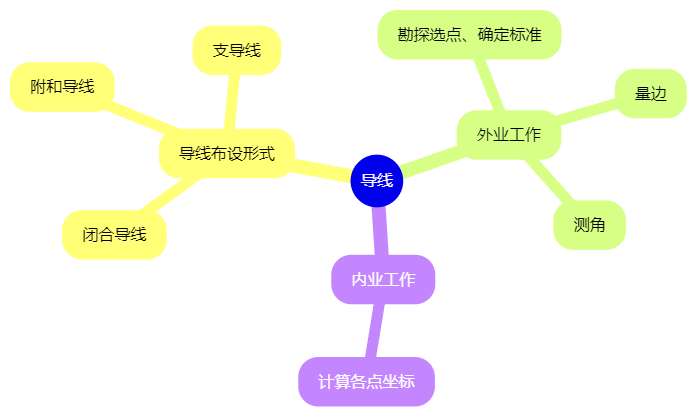
\includegraphics[width=0.75\textwidth]{./figures/10.png}
    \caption{左:控制网的等级;右:导线的布设形式}
\end{figure}

\begin{figure}[H]
    \centering
    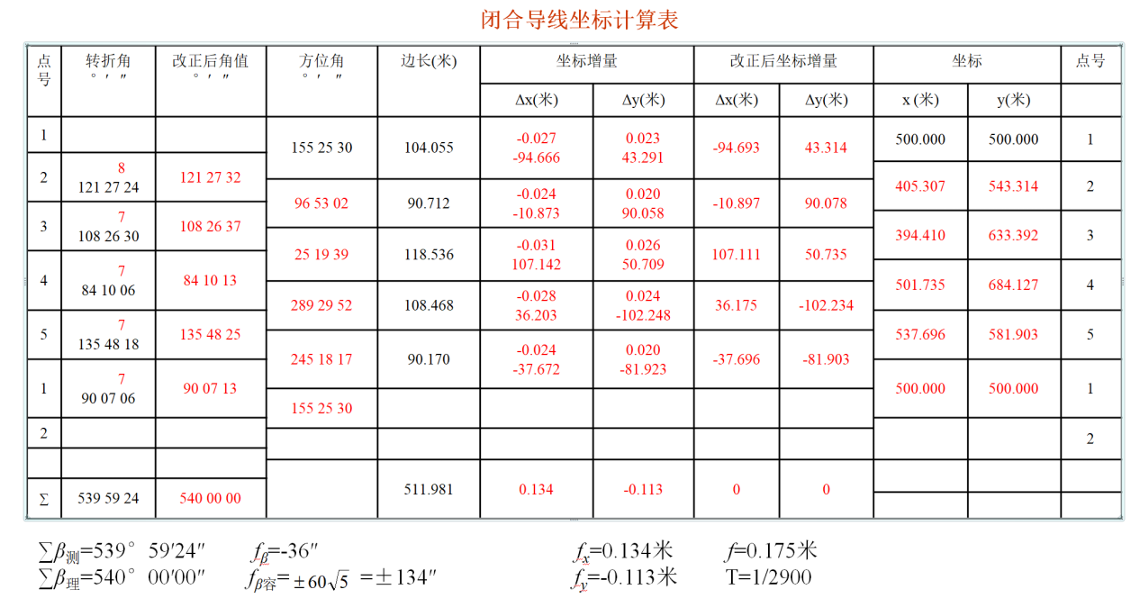
\includegraphics[width=0.9\textwidth]{./figures/11.png}
    \caption{闭合导线计算表}
\end{figure}

{\color{red}这里的角度是随机分配了一个8''的,因为无法整除,正常来说是按角度个数平均分配的。}

在小范围内(一般面积在15平方千米以下)建立的控制网称为小地区控制网。 

全站仪极坐标法定点:通过用全站仪测角和测边,按极坐标法确定点的坐标。
通常用于图根控制测量时加密控制点。

\begin{align*}
x_P &= x_A + D\cos(\alpha_{AB} + \beta) \\
y_P &= y_A + D\sin(\alpha_{AB} + \beta)
\end{align*}

这是在左角的情况下推导的,{\color{red}注意这里是反向的,$\beta$是转角的角度,$\alpha_{AB}$是前一条边的方位角的反角。}

\begin{figure}[H]
    \centering
    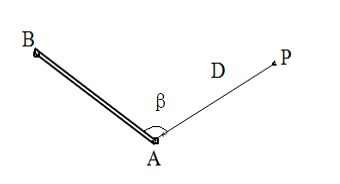
\includegraphics[width=0.6\textwidth]{./figures/12.png}
    \caption{闭合导线计算表}
\end{figure}


高程控制测量常用的方法有水准测量及三角高程测量。电磁波测距三角高程测
量可以代替四等及以下等级的水准测量。 

GNSS 的特点:定位精度高、观测时间短、操作简便、全天候作业、观测点间
无需通视、提供三维坐标。

\newpage

\section*{第八章\quad 地形图的基本知识}

\begin{questions}
    \item 什么是地物和地貌?
    
    \answer{地形包括地物和地貌。地物是指地面上的固定物体,{\color{red}用符号加注记表示},包括人工地物与自然
地物;地貌是指地面高低起伏、倾斜变化的形态。{\color{red}用等高线表示} }。

    \item 什么叫比例尺?什么叫比例尺精度?比例尺精度有何作用?
    
    \answer{地形图上某一直线的图上长度与实地长度之比称为比例尺。比例尺精度是指地形图上0.1毫米所表示的地面实际长度。比例尺越大则精度越高,表示地面状况越详细,同时所消耗的人力、物力
也越大。应选用适当的测图比例尺。

比例尺精度作用为:

(1) 根据比例尺精度,可在测图时确定出地面量距应精确到什么程度。

(2) 根据比例尺精度,可按图上需要表示出实地最小距离来确定测图采用的比例尺。}
    
    \item 什么是等高线平距、等高距?
    
    \answer{
    相邻两条等高线之间的高差称为等高距。
相邻两条等高线之间的水平距离称为等高线平距。
两者的关系为:
\[ i = \frac{h_d}{D} \]
式中 \( i \) 为坡度,\( h_d \) 为等高距,\( D \) 为等高线平距。
    }
\end{questions}

\section*{第八章\quad 知识点补充}
等高线的种类:

\begin{enumerate}
    \item \textbf{首曲线}:按规定等高距测绘的等高线,用 $0.15\,\mathrm{mm}$ 粗的实线表示。
    \item \textbf{计曲线}:从零米起算,每隔四条首曲线加粗描绘的一条等高线,用 $0.3\,\mathrm{mm}$ 粗的实线表示。
    \item \textbf{间曲线}:以二分之一等高距描绘的等高线,用长虚线表示。
    \item \textbf{助曲线}:以四分之一等高距描绘的等高线,用短虚线表示。
\end{enumerate}

几种典型地貌的等高线:山头与洼地的等高线是一组封闭的曲线;山脊的等高
线表现为一组凸向低处的曲线;山谷的等高线表现为一组凸向高处的曲线;鞍部的等
高线的特点是在一圈大的闭合曲线内套有两组小的闭合曲线。 

等高线的基本特性:

\begin{enumerate}
    \item 同一条等高线上的各点高程相等。
    \item 等高线为封闭曲线。
    \item 除陡崖或悬崖外,不同高程的等高线不相交。
    \item 等高线与地性线垂直。
    \item 同一幅图内,等高距相同。
\end{enumerate}

\begin{figure}[H]
    \centering
    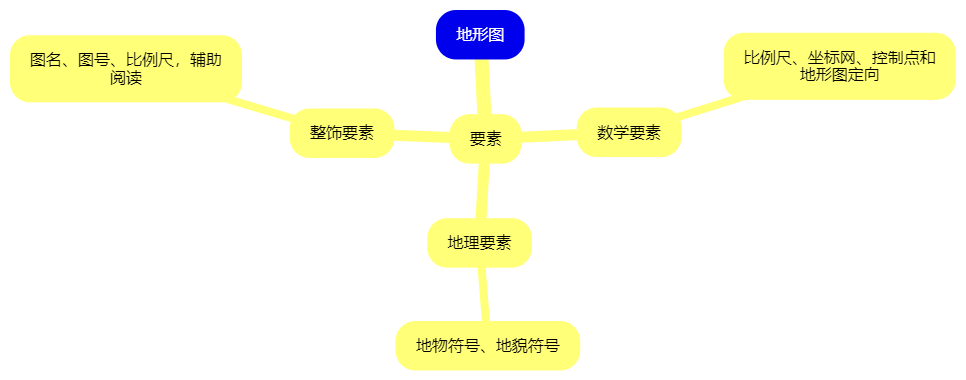
\includegraphics[width=0.8\textwidth]{./figures/13.png}
    \caption{地形图要素}
\end{figure}
\newpage

\section*{第九章\quad 地形图的测绘}

\begin{questions}
    \item 地形测图时,应怎样选择碎部点?
    \answer{对于地物选择能反映地物平面形状的特征点;对 于 地貌应选择山顶、鞍部、
山脊、山谷、山脚等坡度及方向变化处的地貌特征点作为碎部点,地貌用等高线表示。并在
实测的碎部点注上高程。}
    \item 大比例尺数字地图的作业方法有哪些?
    \answer{大比例尺地形测图,根据数据采集方式不同,建立大比例尺数字地图的作业方法通常有以下三种:
(1)现有地图的数字化方法;( 2)基于影像的数字化方法;( 3)地面数字测图方法。

这三种方法的含义分别是:

(1)现有地图的数字化方法:将纸质地图或扫描图像进行矢量化处理,提取地物信息,生成数字地图。

(2)基于影像的数字化方法:利用遥感影像或航拍影像,通过影像识别技术提取地物信息,生成数字地图。

(3)地面数字测图方法:通过全站仪、GPS等测量设备,直接在地面进行测量,获取高精度的地物信息,生成数字地图。

}


\end{questions}

\section*{第九章\quad 知识点补充}

使用测绘仪器测绘地形图的工作称为地形测图。 

地形图测绘是在控制测量工作之后,以控制点为测站,测定其临近的地物、地
貌点的特征点的平面位置与高程,并根据地形图图式规定的线划和符号,将它们表示
在地形图上。

地形图测绘,可采用平板测图、全站仪测图、GPS-RTK测图等方法。 

\begin{enumerate}
    \item 平板测图:采用量角器和钢尺
    \item 全站仪测图:采用全站仪
    \item GPS-RTK测图:采用GPS系统完成测图
\end{enumerate}

大比例尺数字地图的建立分为三个阶段:数据采集、数据处理和地图数据的输
出。

\newpage

\section*{第十一章\quad 施工测量基本工作 }

\begin{questions}
    \item 施工放样的基本工作是什么?
    \answer{放样指的是根据设计图纸,将图纸上的尺寸、形状和位置等信息,准确地标注或描绘到实际施工现场或材料上的过程。
    
    包括测设已知水平距离、测设已知水平角、测设已知高程。
    }
    
    \item 测设点位的方法有哪几种?各适用于什么场合?
    \answer{测设方法主要有:直角坐标法、极坐标法、角度交会法、距离交会法和全站
仪测设法。

\begin{itemize}
    \item 直角坐标法:测点周围已有多个控制点且坐标已知,适合平面开阔、坐标关系明确的区域。
    \item 极坐标法:适用于地面平坦且距离较短的场合(因为极坐标法只要一个参考点)。
    \item 角度交会法:需测设的点位与已知控制点相距较远或不便于量距时。
    \item 距离交会法:当需测设的点位与已知控制点相距较近(小于一尺段)且测设现场较平坦。
    \item 全站仪测设法:适用于各种场合,当距离较远、地势复杂时尤为方便。
\end{itemize}
}

    \item 设 I、J 为控制点,已知 \(X_I = 158.27\) 米,\(Y_I = 160.64\) 米,\(X_J = 115.49\) 米,\(Y_J = 185.72\) 米,A 点的设计坐标为 \(X_A = 160.00\) 米,\(Y_A = 210.00\) 米,试分别计算用极坐标法、角度交会法及距离交会法测设 A 点所需的放样数据。

    \answer{
    1. 极坐标法(以点 \(I\) 为极点)

坐标差:
\[
\Delta X = X_A - X_I = 160.00 - 158.27 = 1.73\,\text{m}
\]
\[
\Delta Y = Y_A - Y_I = 210.00 - 160.64 = 49.36\,\text{m}
\]

距离:
\[
s = \sqrt{(\Delta X)^2 + (\Delta Y)^2} = \sqrt{1.73^2 + 49.36^2} = \sqrt{2.99 + 2436.50} = \sqrt{2439.49} \approx 49.39\,\text{m}
\]

方向角(这里是第一象限的,如果不是得补角,比如说第三象限和第二象限要加$180^\circ$):
\[
\alpha = \arctan \frac{\Delta Y}{\Delta X} = \arctan \frac{49.36}{1.73} \approx \arctan(28.53) =88.00^\circ
\]

\vspace{1em}
\textbf{极坐标法放样数据:}  
\[
\text{起点:} I, \quad \text{距离} = 49.39\,\text{m}, \quad \text{方位角} = 88.00^\circ
\]

2. 角度交会法

计算点 \(I\) 到点 \(J\) 的方位角:
\[
\Delta X_{IJ} = X_J - X_I = 115.49 - 158.27 = -42.78
\]
\[
\Delta Y_{IJ} = Y_J - Y_I = 185.72 - 160.64 = 25.08
\]
\[
\alpha_{IJ} = \arctan \frac{|\Delta X_{IJ}|}{\Delta Y_{IJ}} = \arctan \frac{42.78}{25.08} = 59.6^\circ
\]

由于 \(\Delta X_{IJ} < 0\) 且 \(\Delta Y_{IJ} > 0\),点 \(J\) 在第二象限,方位角为:
\[
\alpha_{IJ} = 180^\circ - 59.6^\circ = 120.4^\circ
\]

点 \(I\) 到点 \(A\) 的方位角:
\[
\alpha_{IA} = 88.00^\circ \quad \text{(同极坐标法)}
\]

点 \(J\) 到点 \(A\) 的方位角:
\[
\Delta X_{JA} = X_A - X_J = 160.00 - 115.49 = 44.51
\]
\[
\Delta Y_{JA} = Y_A - Y_J = 210.00 - 185.72 = 24.28
\]
\[
\alpha_{JA} = \arctan \frac{24.28}{44.51} = \arctan(0.54) = 28.4^\circ
\]

\vspace{1em}
\textbf{角度交会法放样数据:}  
\[
\text{点 } I: \alpha_{IA} = 88.00^\circ, \quad \text{点 } J: \alpha_{JA} = 28.4^\circ
\]

3. 距离交会法

点 \(A\) 到点 \(I\) 的距离:
\[
d_{AI} = 49.39\,\text{m} \quad \text{(同极坐标法)}
\]

点 \(A\) 到点 \(J\) 的距离:
\[
d_{AJ} = \sqrt{(X_A - X_J)^2 + (Y_A - Y_J)^2} = \sqrt{44.51^2 + 24.28^2} = \sqrt{1981.20 + 589.47} = \sqrt{2570.67} \approx 50.70\,\text{m}
\]

\vspace{1em}
\textbf{距离交会法放样数据:}  
\[
d_{AI} = 49.39\,\text{m}, \quad d_{AJ} = 50.70\,\text{m}
\]


    }
\end{questions}

\section*{第十一章\quad 知识点补充}

各种工程在施工阶段所进行的测量工作称为施工测量。 施工测量的主要内容包括:建立施工控制网、放样、检查验收测量、变形观测、
竣工测量等。 

铅垂线的测设,就是将点位沿竖直方向向上或向下传递,可用经纬仪投测法、
垂线法、激光铅垂仪投测法、光学垂准仪投测法等方法。 

全站仪可采用极坐标法或坐标法测设点位。

%=================== 答案部分 ===================


\end{document}
%================= 结束 =================%
